% Please do not change the document class
\documentclass{scrartcl}

% Please do not change these packages
\usepackage[hidelinks]{hyperref}
\usepackage[none]{hyphenat}
\usepackage{setspace}
\doublespace

% You may add additional packages here
\usepackage{amsmath}
\usepackage{graphicx}
\usepackage{url}

% Please include a clear, concise, and descriptive title
\title
{
What to consider when porting a console or PC game to a mobile device
}

% Please do not change the subtitle
\subtitle{COMP160 - Software Engineering Essay}

% Please put your student number in the author field
\author{Student number: 1607539}

\begin{document}

\maketitle

\abstract
{
There is a lucrative market for mobile games, and many console and PC game developers port their software to phones and tablets.  This essay will describe the technical aspects of porting, and will examine three games that have been ported from a console or PC to a mobile device.  By comparing the original version against the ported version of the Bioshock, Grand Theft Auto (GTA), and Final Fantasy (FF) series, conclusions will be drawn on the pitfalls regarding portability to mobile devices in game development.

\section*{Introduction}

Given the dominance of the x86 architecture, common application programming interfaces (APIs) through widely used software like DirectX, and industry standard hardware: high definition monitors, qwerty keyboards, and twin stick console controllers, porting software between like machines can be cheap. However, with the market for mobile games worth nearly a quarter (\pounds995.1 million) of the entire UK games industry in 2016 \cite {UKIE2017}, console and PC game developers must consider allowing and easing portability to a mobile system. A system whose hardware, software, input, and output likely differ greatly from the original target platform.  The mobile gamer demography also differs greatly from the console or PC gamer in what style of games they play, so a game developer must objectively decide whether even a successful port would sell enough to justify the process.

\section*{Input}

As with many other proper programming practices, allowing flexibility with the hardware input and output of a game during development must be considered from the start.  Most game building engines, including Unity and Epic, offer input mappings so that custom events can be created and then later mapped to controls.  Not only does this encourage a level of abstraction when developing a controller program which separates the events from the processes, but is integral to the process of porting a game to another system whose control scheme is different. The software will obviously not automatically translate a keyboard's space bar press into a console controller's jump input. But were a jump event defined in the upper levels of the program, a developer can assign that event to any number of different inputs. It is important to note that if no such input event customisation options are available, in PyGame for example, then one should be created, through a dictionary structure or similar.

Whilst many modern controllers have more than ten buttons and two joysticks, mobile devices can only be relied to have a touchscreen in common. Any buttons are proprietary and are used to change the volume or lock the device.  A touch on a touchscreen can have five different states; started, ended, moved, stationary, or cancelled (if a call were received on a smartphone mid game) and the developer must recreate complex and intuitive controls using some amount of simultaneous touch states. All three of the studied games relied upon a virtual joystick for movement mapped to the touch input on the lower left of the screen. It must be an obvious solution given the standard controller convention and that input mappings exist for joystick axis and amounts, and whilst this may work fine for the slow paced FF franchise; Bioshock and GTA rely on precision and reflexes.  GTA has made some attempt to patch this inaccuracy with an enemy lock on and location specific pop up interfaces, but the result is ineffective.

When touch screen controls are being used, then nothing critical to the player experience should be placed on screen in that space. GTA mimics car chases by showing the chasing car appear into the lower left or right portion of the screen. On a smartphone, this detail is where the player's hands must be to move the virtual joystick so the experience suffers.

In an interview with Satoru Iwata on the Wii launch website, Akio Ikeda, who was responsible for the accelerometer hardware on the Wii, said ``Of course, when playing a game, the nearest thing to the player is the controller. The controller should therefore be regarded as an extension of the player rather than as part of the console. I always bear in mind the importance of the fact that the player will have far more contact with the controller and UI than the console itself.'' While these comments were obviously made in relation to a console, the importance of interface is particularly relevant to mobile phones \cite {gilbertson2008using}.

Game developers must consider whether their control scheme can be replicated on a touch device, if it must be rewritten, or how the game can be balanced if either is inadequate.

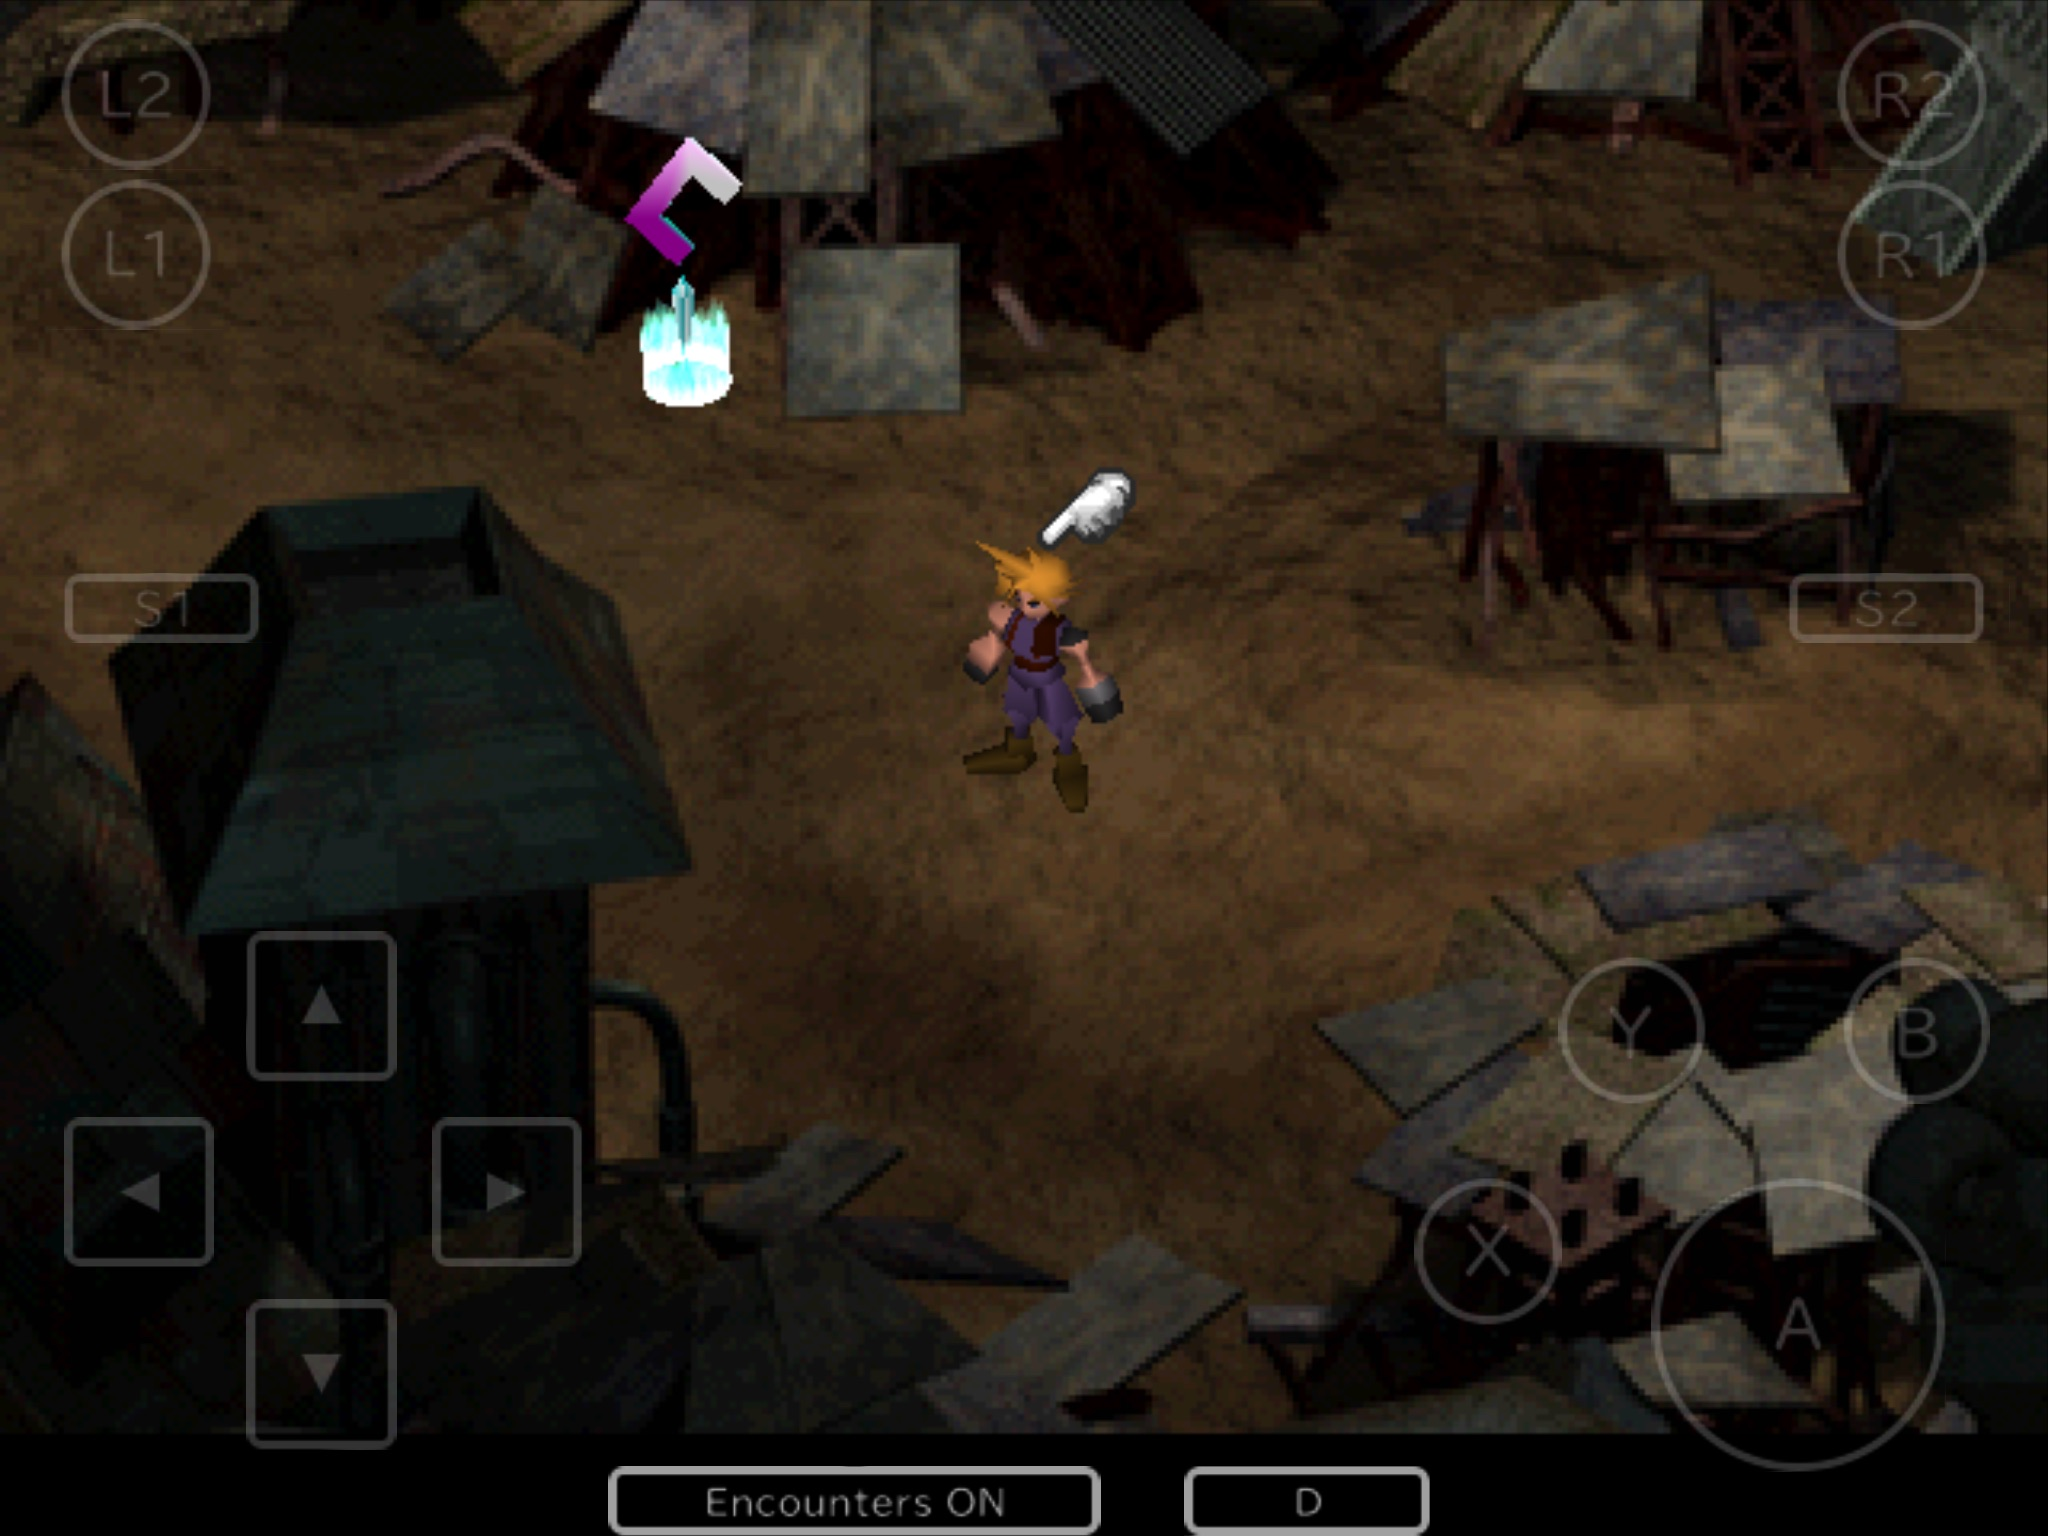
\includegraphics[scale = 0.18]{FF7_IOS_Controls}{
    \emph{Final Fantasy VII} on IOS, on screen controls.
}

\section*{Output}

With differing screen resolutions, a game developer must ask; will my game scale properly from a window to full screen? Or how does dpi and aspect ratios affect the user interface (UI)?  Intuitive designers will often anchor UI to respective corners of a screen, but what if the game was ported to a system with a screen smaller than the UI? The image may scale disproportionately or overlap itself.

Whilst many console gamers boast 1080p displays larger than 50'', were the UI scaled similarly to a 5'' 1080p smartphone then the UI itself, at least the available size in the viewport, would also shrink by a factor of ten. Detailed menu screens as found in FFVI become much harder to read than their console counterparts, in particular within the status or Sabin's Blitz options screens.  GTA has implemented large button menu screens for smaller devices, but has left much of the in game writing, such as in the map, at its original ratio.  A good gaming experience requires a lot from the user interface. It should be convenient, reliable, and usable so that the player can concentrate on playing the game and enjoying it instead of struggling with the user interface \cite {korhonen2006playability}.\\

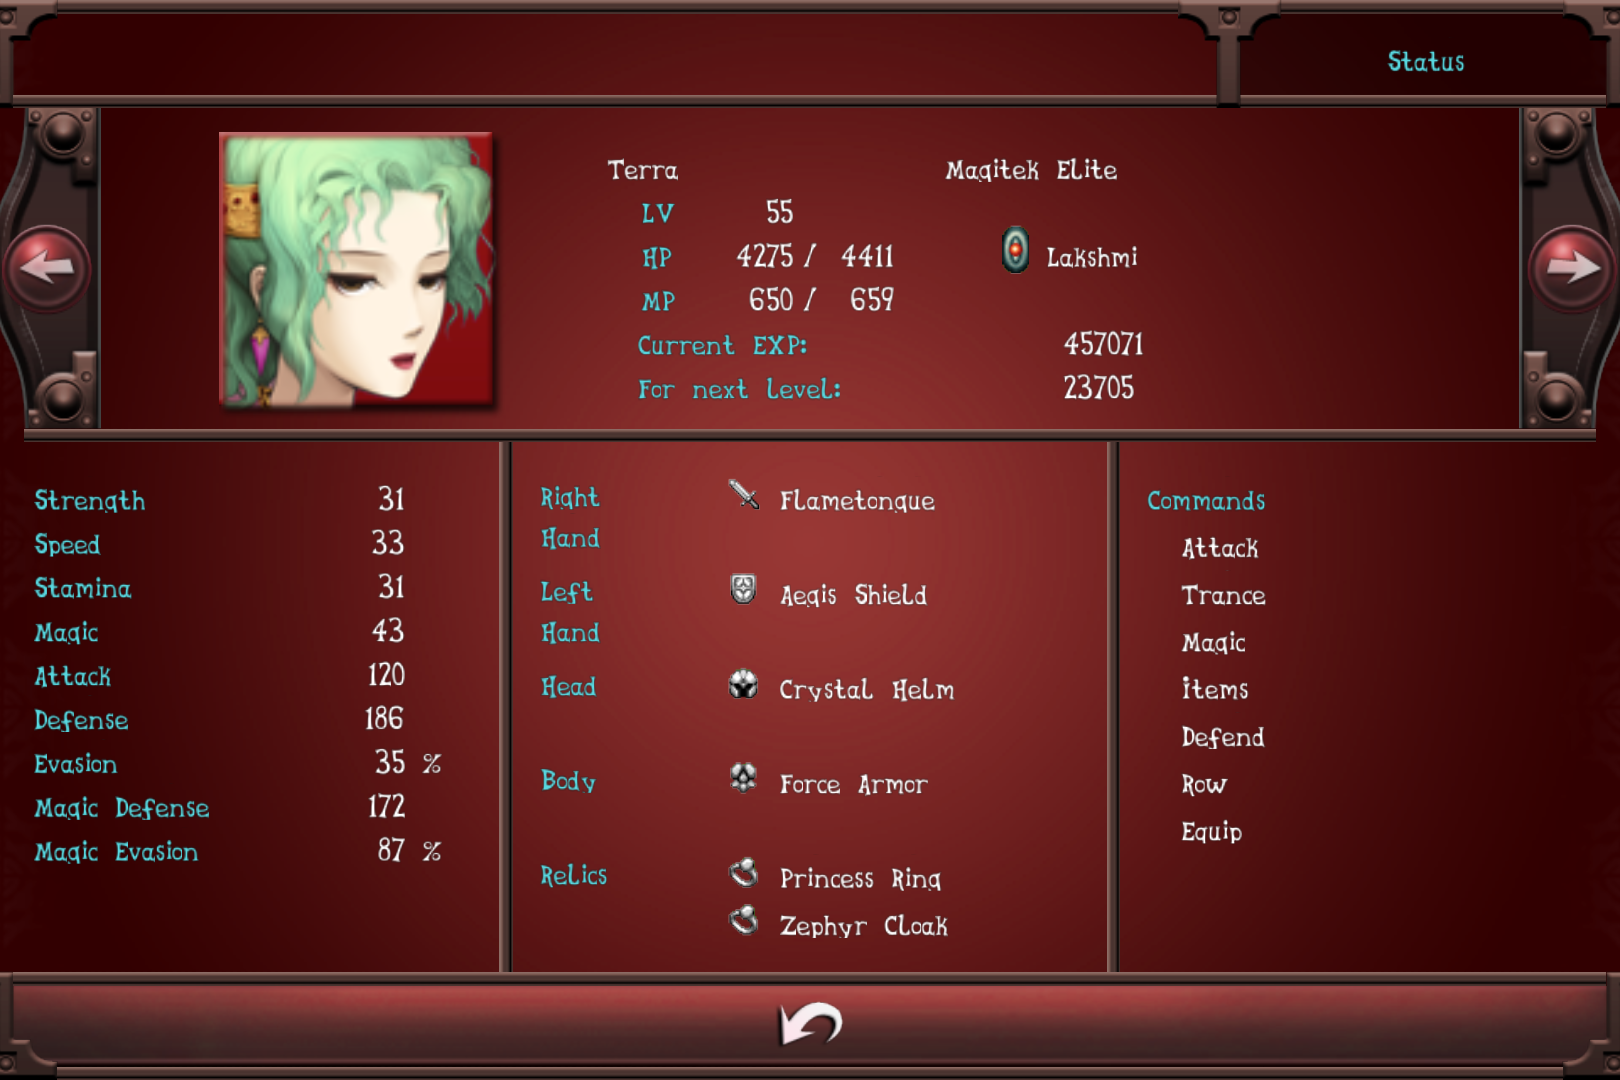
\includegraphics[scale = 0.12]{FFVI_iOS_Status_Menu}
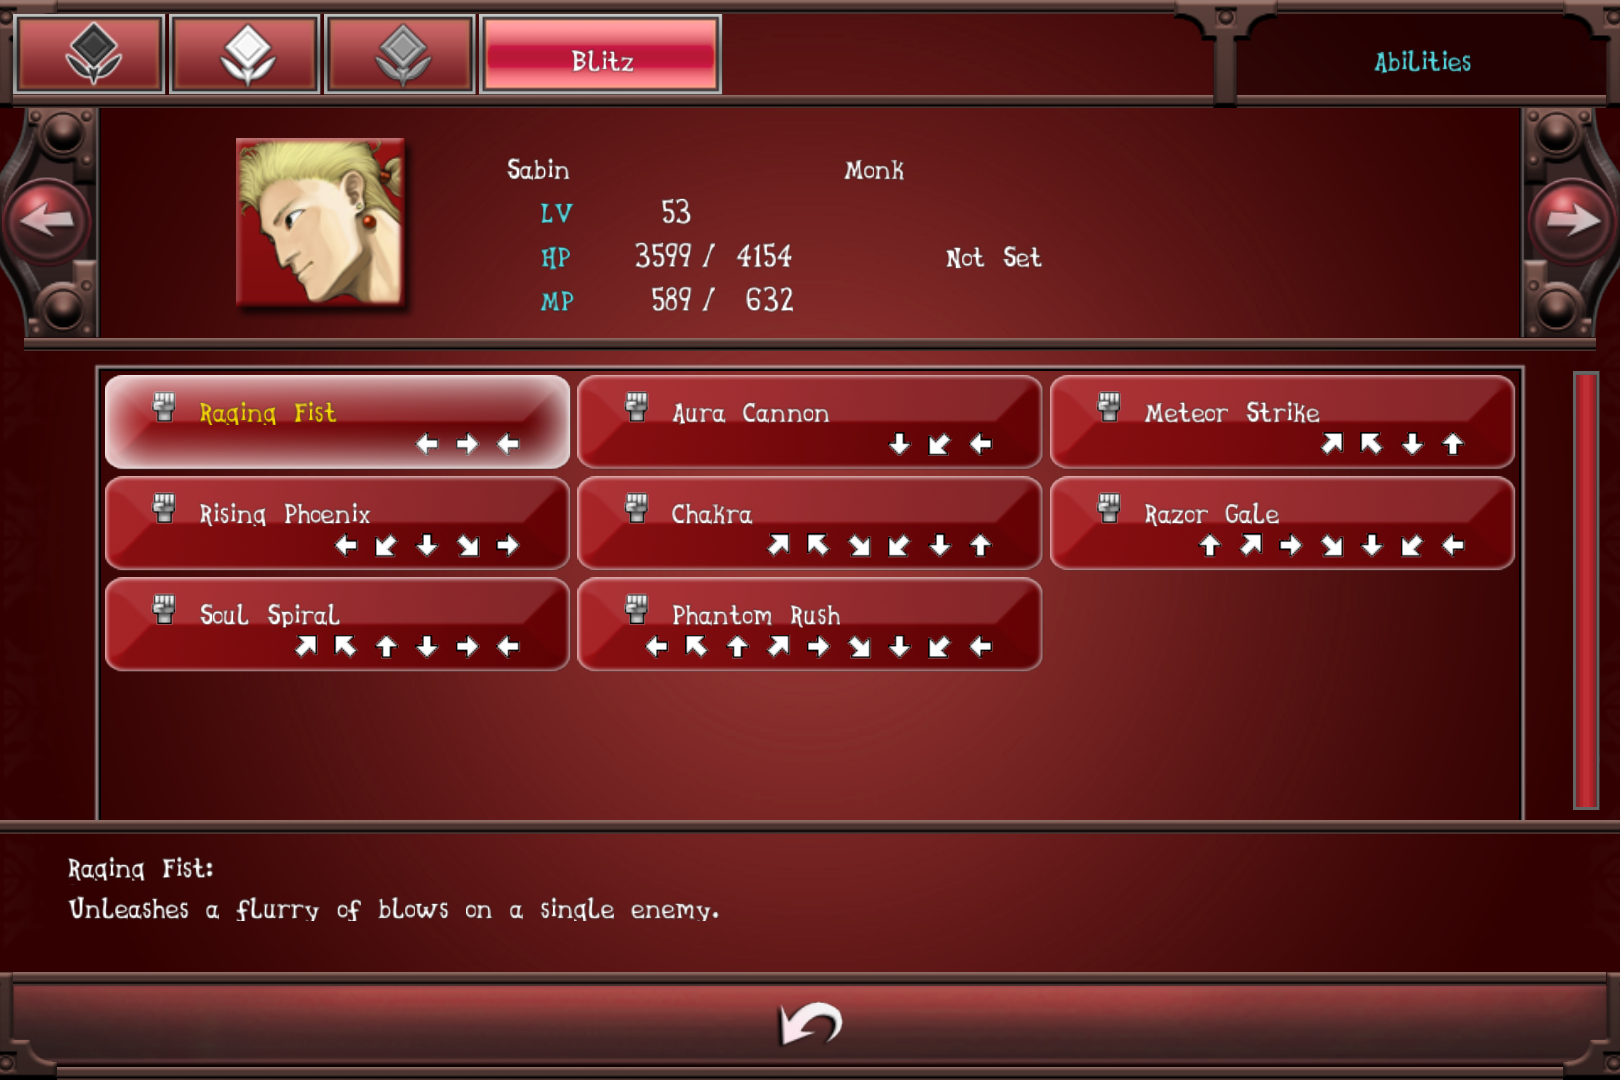
\includegraphics[scale = 0.12]{FFVI_Android_Blitz_Menu}{
    \emph{Final Fantasy VI} on IOS, character status menu (left), and on Android, Sabin's Blitz menu (right).\\
}


\includegraphics[scale = 1.05]{GTASanAndreas_IOS_Start_menu}
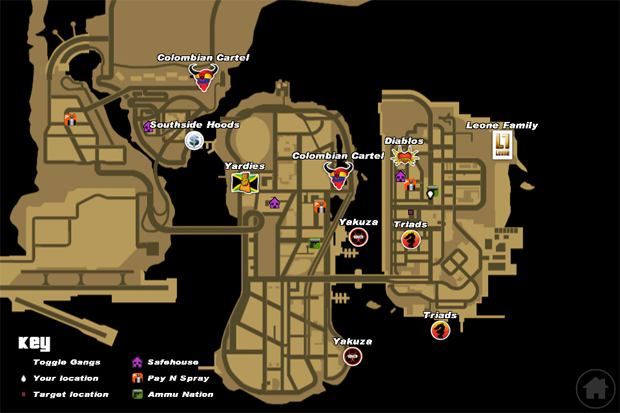
\includegraphics[scale = 0.27]{GTAIII_IOS_Map}{
    \emph{Grand Theft Auto III} on IOS, start menu (left), and map screen (right).
}

\section*{Software}

Given that many game developers can work from a multi platform game engine like Unity or Epic, compiling a program for a mobile system is straightforward.  For those who do not, the process is more difficult.  When Blitworks faced porting 'Fez' to the Playstation 3 the most difficult challenge they had was that the original Fez game was written in C\#, and there was no C\# support for PlayStation platforms when they started the port, so they faced the big decision of trying to port the whole Mono runtime or to convert the game to C++ \cite {gamasutra2014}.

Without relying upon an established compiler to translate the project it is essential to be familiar with the target platforms software development kit (SDK).  Existing platforms have taken different approaches when it comes to sharing their SDK with developers. Some have chosen to restrict access as much as possible, whereas others have chosen to disclose the entire source code of their SDK and OS \cite {holzer2009trends}.

Like consoles, mobile devices must suffer major software updates at least once a year \cite {Android2017History}.  However, unlike most gaming centric consoles, mobile device software updates can have drastic effects upon a games ability to run.  In fact, because of software compatibility issues, Bioshock has been indefinitely removed from the IOS app store.

There is little that can be done about this.  However, working within an established multi platform engine will offer some insurance against SDK changes affecting existing libraries.

\section*{Hardware}

Greatly differing or inadequate resources on the target platform are the cause of many failed ports. Despite the PS3 being the most technologically advanced video game console of the seventh generation \cite {ofek2008sony}, developing required a lot of effort, source code developed for the CELL processor is not portable at all on other architectures \cite {buttari2007limitations}, so developers would concentrate on the Xbox 360 and port to the ps3 later.  Bayonetta suffered famously from this port, with load times between levels far longer than the original \cite {Kotaku2010Bayonetta}.

For a mobile device, despite the sizeable RAM and powerful ARM CPU able to generate complex 3D environments, the battery usage of a smaller device can often be a key concern.  The compute and memory intensive nature of 3D games translates to substantially high power consumption in the mobile platforms \cite {pathania2014integrated}.  Intensive processes like dynamic colliders and particle effects in general must be avoided, approximated, or minimised in their use. Bioshock has had to make the largest change in this respect, approximating the particle effects for the plasmids for the mobile version.\\

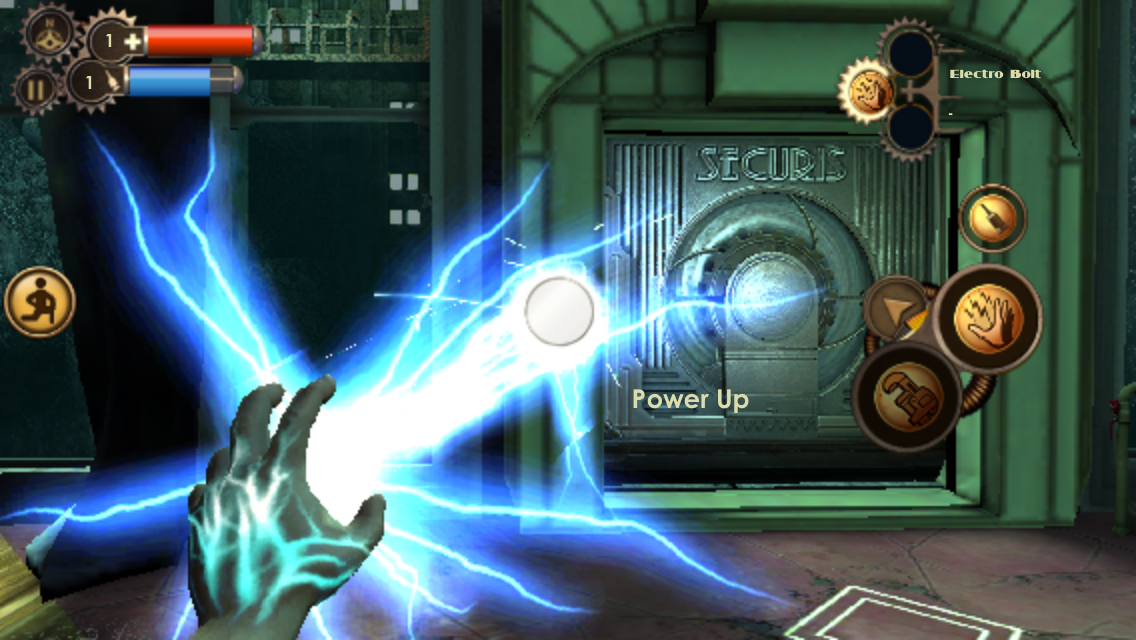
\includegraphics[scale = 0.3]{Bioshock_IOS_Plasmid}\\{
    \emph{Bioshock} on IOS, plasmids.
}\\

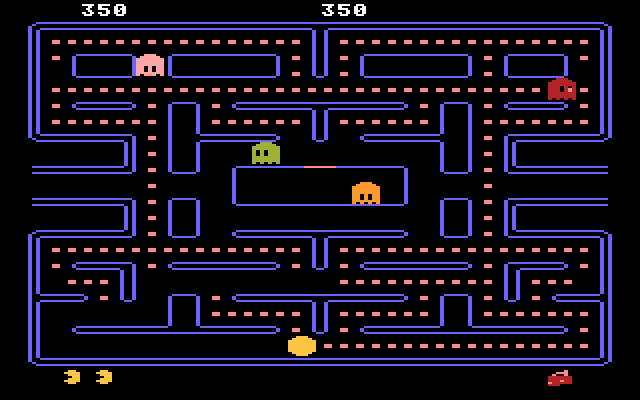
\includegraphics[scale = 0.3]{PacMan_Original}
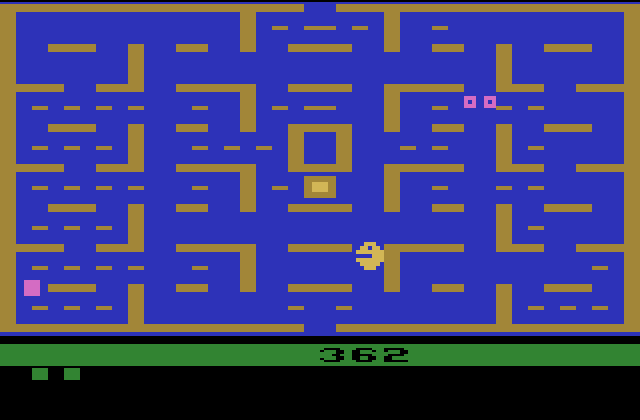
\includegraphics[scale = 0.285]{PacMan_(1982)_Atari_Port}{
    \emph{PacMan} on the Atari 5200 (left), compared to the famously poor Atari 2600 port (right).
}

\section*{The Game}

All of the examined games were vast in their original scope with playthroughs requiring hundreds of hours to complete; hardly suited to a casual player passing time on a commute.  So why do consumers buy them if not to complete them?  When originally released, all three of the games were at the forefront of what was possible in computing.  There is pride in being able to carry these once masterpieces around in your pocket, to boast to your friends about what your latest smartphone can achieve.

Some games can be fun over time without ever advancing through the story; GTA allows a considerable amount of exploration from very early on, whilst FF7 on mobile even includes a MaxStats setting in the options, setting every character to have 9,999 hitpoints and 999,999,999 gil, acknowledging the idea that players don't want a faithful replication of the original version with all of its challenges.

Older games which rely less on visuals and sound suit a smaller device.  FF and GTA have even since had a graphical upgrade since their original versions.  Conversely Bioshock, a game built on story and atmosphere, is a peculiar choice for a mobile setting.  It is difficult to immerse a player in the underwater ruins of Rapture from a small screen with poor audio capabilities.

When porting a large game to a mobile device it is important to avoid frustrating moments.  Either tailoring the game to suit shorter sessions with more frequently available save points, or overpowering the player so that frustrating deaths and subsequent replays are avoided.\\

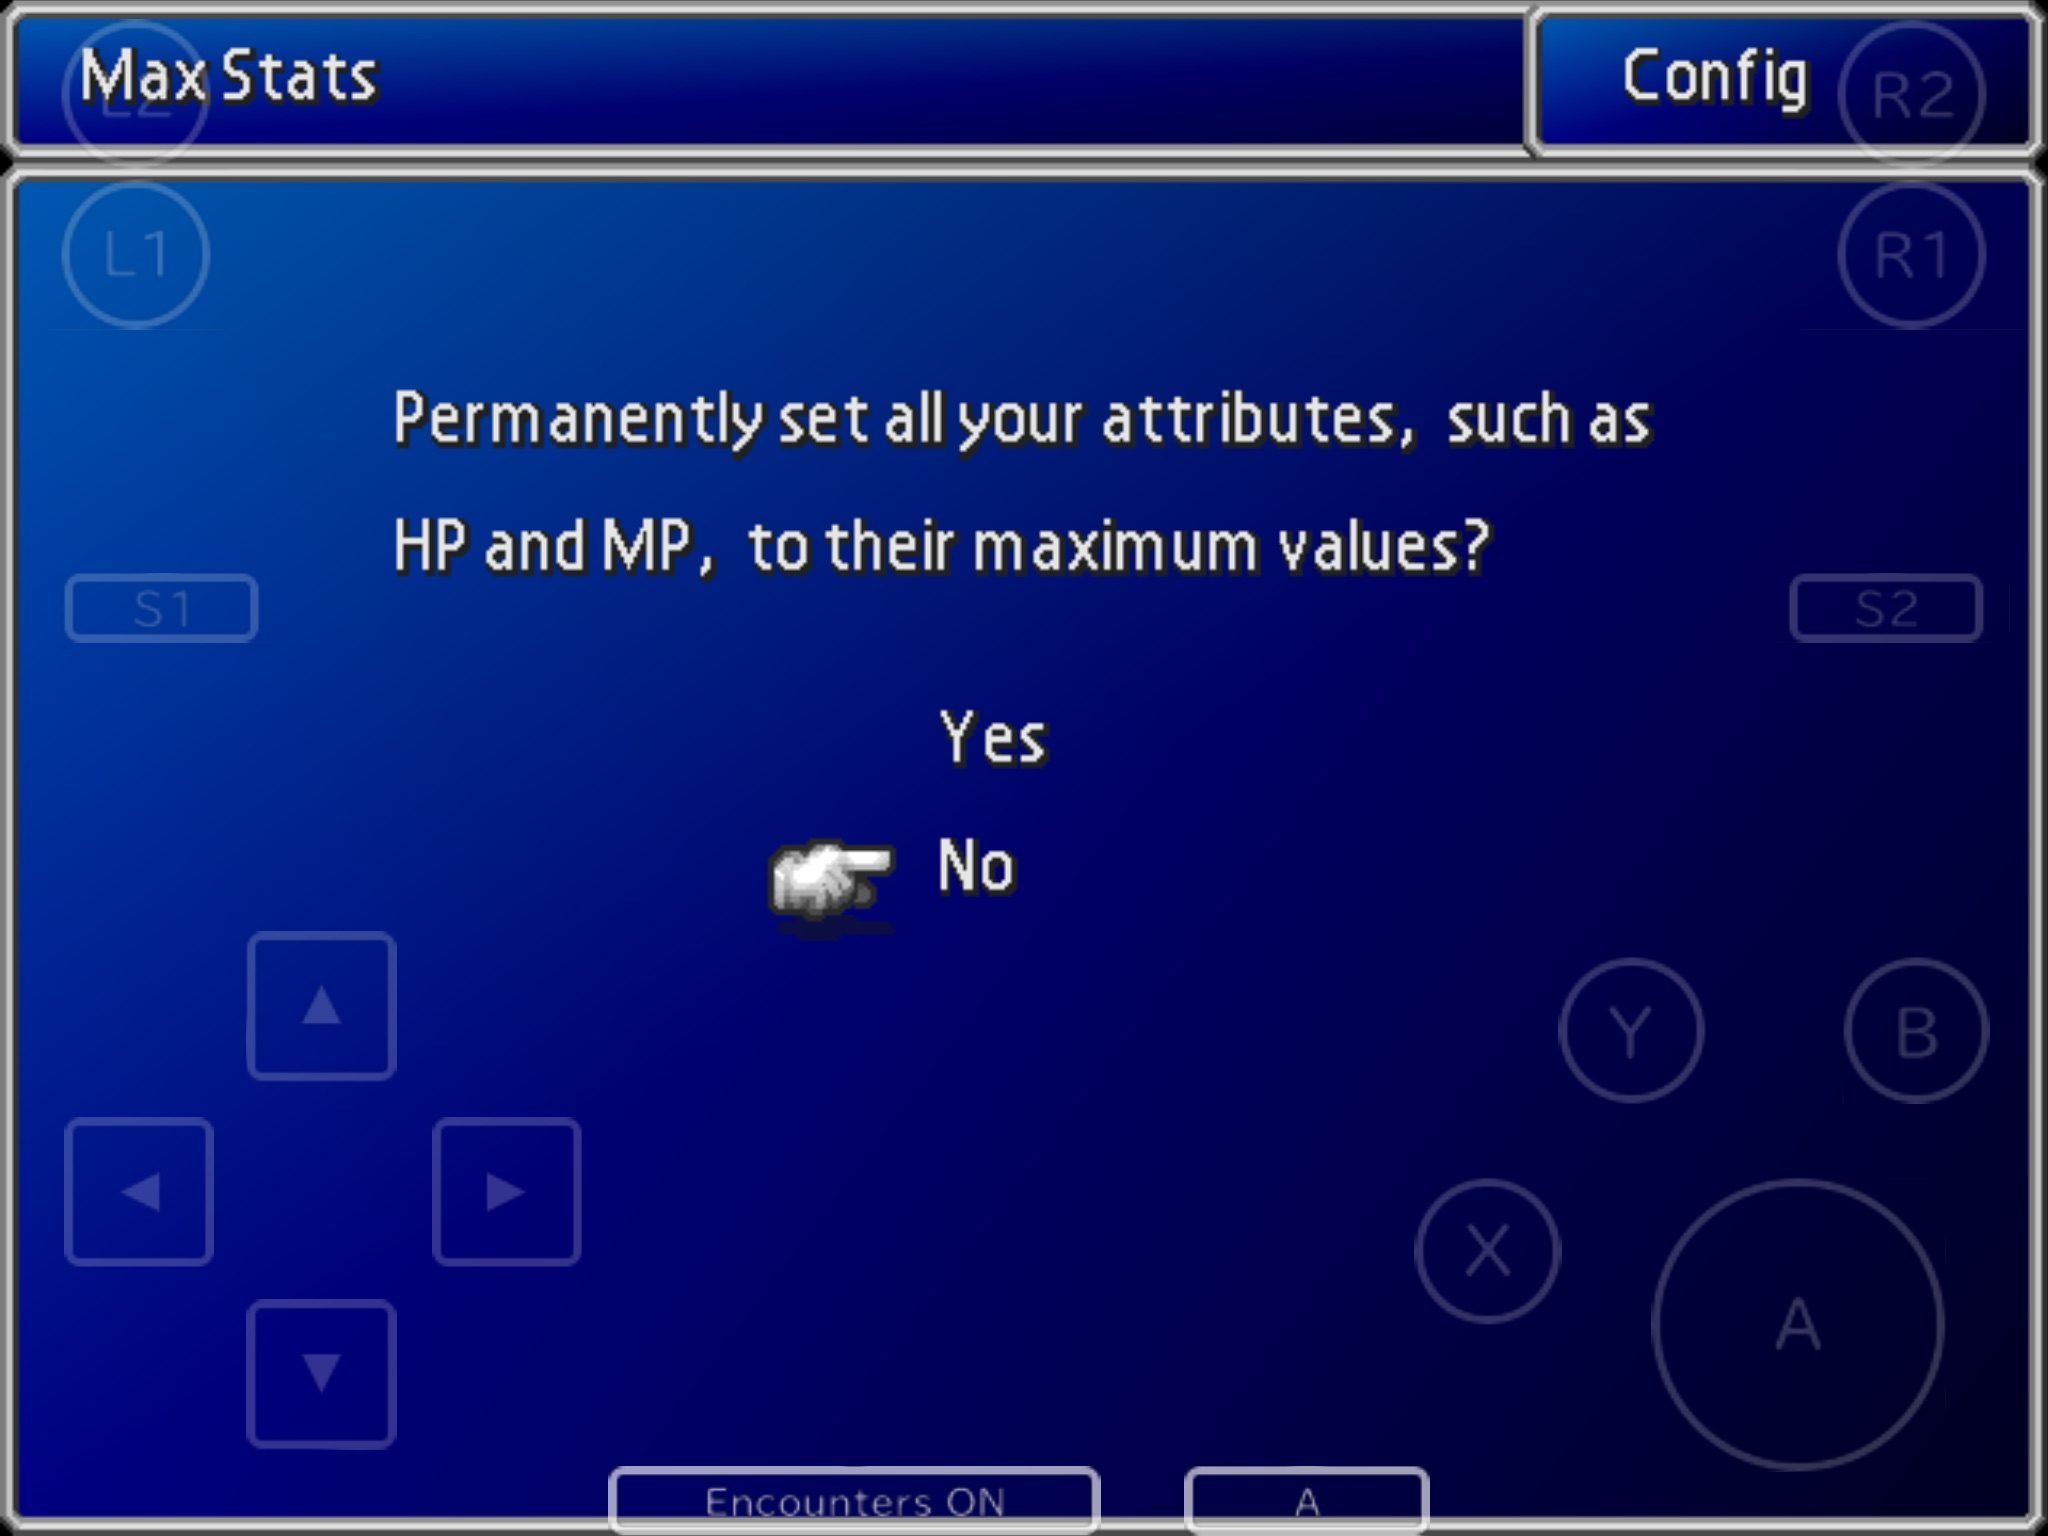
\includegraphics[scale = 0.18]{FF7_IOS_MaxStats}{
    \emph{Final Fantasy VII} on IOS.
}

\section*{Conclusion}

This essay has identified key factors to consider when developing a game that is portable to mobile devices.  Namely to concentrate on the players ease of input, output, and to maximise fun over a short session, even if this counters the original game's style or challenge.

\bibliographystyle{ieeetran}
\bibliography{references}

\end{document}
